% ============================================================================
% GOV 2001: Probability Foundations
% Lecture 01a - Week 1, Day 1
% Spring 2026
% ============================================================================

\documentclass[aspectratio=169, 11pt]{beamer}

% ============================================================================
% PREAMBLE: Gov 2001 House Style
% ============================================================================

% --- Typography ---
\usepackage[T1]{fontenc}
\usepackage{libertine}                    % Main text: Linux Libertine
\usepackage[libertine]{newtxmath}         % Math: matching libertine style
\usepackage{inconsolata}                  % Monospace: Inconsolata
\usepackage{microtype}                    % Subtle typographic improvements

% --- Colors ---
\usepackage{xcolor}

% Primary palette: muted, professional
\definecolor{harvardcrimson}{HTML}{A51C30}   % Harvard crimson (used sparingly)
\definecolor{slate}{HTML}{4A5568}            % Primary text color
\definecolor{charcoal}{HTML}{2D3748}         % Headings, emphasis
\definecolor{forest}{HTML}{276749}           % Accent (theorems, key terms)
\definecolor{ocean}{HTML}{2B6CB0}            % Secondary accent (links, refs)
\definecolor{warmgray}{HTML}{718096}         % De-emphasized text
\definecolor{cream}{HTML}{FFFAF0}            % Highlight backgrounds
\definecolor{lightgray}{HTML}{F7FAFC}        % Subtle backgrounds

% --- Beamer Theme Configuration ---
\usetheme{default}
\usecolortheme{default}

% Remove navigation symbols
\setbeamertemplate{navigation symbols}{}

% Frame title
\setbeamertemplate{frametitle}{%
  \vspace{0.5em}
  \textcolor{charcoal}{\large\bfseries\insertframetitle}
  \par\vspace{0.2em}
  \textcolor{warmgray}{\small\insertframesubtitle}
}

% Slide background
\setbeamercolor{background canvas}{bg=white}

% Title page styling
\setbeamercolor{title}{fg=charcoal}
\setbeamercolor{subtitle}{fg=warmgray}
\setbeamercolor{author}{fg=slate}
\setbeamercolor{institute}{fg=warmgray}
\setbeamercolor{date}{fg=warmgray}

% Body text
\setbeamercolor{normal text}{fg=slate}
\setbeamercolor{structure}{fg=forest}

% Itemize styling
\setbeamertemplate{itemize items}[circle]
\setbeamercolor{itemize item}{fg=forest}
\setbeamercolor{itemize subitem}{fg=slate}
\setbeamertemplate{itemize subitem}[triangle]

% Blocks
\setbeamercolor{block title}{fg=white, bg=forest}
\setbeamercolor{block body}{fg=slate, bg=lightgray}
\setbeamertemplate{blocks}[rounded][shadow=false]

% Alerts
\setbeamercolor{alerted text}{fg=harvardcrimson}

% Footline
\setbeamertemplate{footline}{%
  \hbox{%
    \begin{beamercolorbox}[wd=0.33\paperwidth,ht=2.5ex,dp=1ex,left]{author in head/foot}%
      \hspace{1em}\textcolor{warmgray}{\tiny Gov 2001}
    \end{beamercolorbox}%
    \begin{beamercolorbox}[wd=0.34\paperwidth,ht=2.5ex,dp=1ex,center]{title in head/foot}%
      \textcolor{warmgray}{\tiny\insertshortauthor}
    \end{beamercolorbox}%
    \begin{beamercolorbox}[wd=0.33\paperwidth,ht=2.5ex,dp=1ex,right]{date in head/foot}%
      \textcolor{warmgray}{\tiny\insertframenumber\,/\,\inserttotalframenumber}\hspace{1em}
    \end{beamercolorbox}%
  }%
}

% --- Math and Symbols ---
\usepackage{amsmath, amssymb, amsthm}
\usepackage{mathtools}
\usepackage{bm}                           % Bold math symbols

% Custom math operators
\DeclareMathOperator{\E}{\mathbb{E}}
\DeclareMathOperator{\Var}{Var}
\DeclareMathOperator{\Cov}{Cov}
\DeclareMathOperator{\Corr}{Corr}
\DeclareMathOperator{\plim}{plim}
\newcommand{\indep}{\perp\!\!\!\perp}
\newcommand{\Prob}{\mathbb{P}}
\newcommand{\R}{\mathbb{R}}

% --- Graphics ---
\usepackage{graphicx}
\usepackage{tikz}
\usetikzlibrary{arrows.meta, positioning, shapes, calc, decorations.pathreplacing}

% --- Tables ---
\usepackage{booktabs}
\usepackage{array}
\usepackage{colortbl}

% --- Hyperlinks ---
\usepackage{hyperref}
\hypersetup{
  colorlinks=true,
  linkcolor=ocean,
  urlcolor=ocean,
  citecolor=forest
}

% --- Custom Commands ---
\newcommand{\highlight}[1]{\textcolor{forest}{\bfseries #1}}
\newcommand{\deemph}[1]{\textcolor{warmgray}{#1}}
\newcommand{\red}[1]{\textcolor{harvardcrimson}{#1}}

% --- Spacing ---
\setlength{\parskip}{0.5em}

% ============================================================================
% DOCUMENT METADATA
% ============================================================================

\title{Probability Foundations}
\subtitle{The Language of Uncertainty}
\author{Scott Cunningham}
\institute{Harvard University \\ Department of Government}
\date{January 26, 2026}

% ============================================================================
\begin{document}
% ============================================================================

\begin{frame}[plain]
\titlepage
\end{frame}

% ----------------------------------------------------------------------------
% WHY START HERE?
% ----------------------------------------------------------------------------

\begin{frame}
\frametitle{Why Start Here?}

\vspace{1em}

\begin{center}
\Large
\textcolor{forest}{\textbf{Today}}: The language of probability
\end{center}

\vspace{1.5em}

Probability is the vocabulary for describing \highlight{populations} and \highlight{uncertainty}.

\vspace{0.5em}

Before we can estimate anything, we need language to describe \emph{what we're trying to learn}.

\vspace{1em}

\deemph{This course takes a ``population-first'' approach: define what you want to know about the population before worrying about estimation.}

\end{frame}

% ----------------------------------------------------------------------------
% PART I: SAMPLE SPACES AND EVENTS
% ----------------------------------------------------------------------------

\begin{frame}
\frametitle{Part I}

\vspace{2em}

\begin{center}
\Huge
\textcolor{charcoal}{\textbf{Sample Spaces and Events}}
\end{center}

\vspace{1em}

\begin{center}
\large
\deemph{The building blocks}
\end{center}

\end{frame}

% ----------------------------------------------------------------------------

\begin{frame}
\frametitle{What Is Probability?}

\vspace{0.5em}

A \highlight{model} for describing uncertainty about outcomes.

\vspace{1em}

\textbf{Three ingredients:}

\vspace{0.5em}

\begin{enumerate}
\item A \highlight{sample space} $\Omega$: all possible outcomes
\vspace{0.3em}
\item An \highlight{event space} $\mathcal{S}$: subsets of outcomes we care about
\vspace{0.3em}
\item A \highlight{probability measure} $\Prob$: assigns numbers to events
\end{enumerate}

\vspace{1em}

\deemph{Together, $(\Omega, \mathcal{S}, \Prob)$ is a \textbf{probability space}.}

\end{frame}

% ----------------------------------------------------------------------------

\begin{frame}
\frametitle{Probability Is a Model}
\framesubtitle{Not a property of the world}

Consider flipping a coin. If you knew \emph{everything}---the exact force applied, the coin's initial orientation, air resistance, the surface it lands on---you could predict exactly whether it lands heads or tails. There's nothing inherently ``random'' about a coin flip.

\vspace{0.3em}

\textbf{So what is probability?}

\vspace{0.3em}

It's a \highlight{model of our uncertainty}, not a feature of physical reality. We use probability because we \emph{don't} know everything---it describes what we believe given our ignorance.

\vspace{0.3em}

This is a key feature of the \highlight{agnostic approach} we take in this course (following Aronow \& Miller). It's worth noting upfront.

\vspace{0.3em}

\begin{center}
\deemph{``All models are wrong, but some are useful.'' --- George Box}
\end{center}

\end{frame}

% ----------------------------------------------------------------------------

\begin{frame}
\frametitle{Sample Space}
\framesubtitle{All possible outcomes}

\vspace{0.5em}

The \highlight{sample space} $\Omega$ is the set of all possible outcomes of a random process.

\vspace{1em}

\textbf{Examples:}

\vspace{0.5em}

\begin{itemize}
\item Coin flip: $\Omega = \{\text{Heads}, \text{Tails}\}$
\vspace{0.3em}
\item Die roll: $\Omega = \{1, 2, 3, 4, 5, 6\}$
\vspace{0.3em}
\item Two coin flips: $\Omega = \{HH, HT, TH, TT\}$
\vspace{0.3em}
\item Temperature tomorrow: $\Omega = \R$ (or some interval)
\end{itemize}

\vspace{1em}

\deemph{The sample space can be finite, countably infinite, or uncountable.}

\end{frame}

% ----------------------------------------------------------------------------

\begin{frame}
\frametitle{Visualizing the Sample Space}
\framesubtitle{The universe of possibilities}

\vspace{0.5em}

\begin{center}
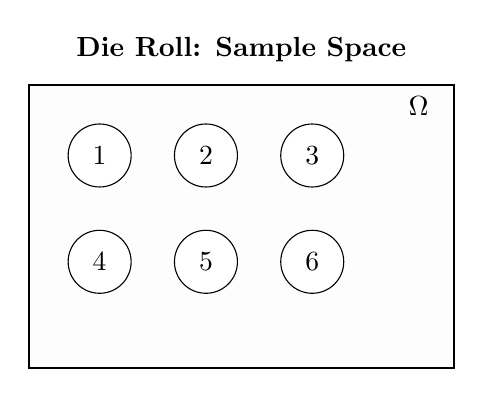
\begin{tikzpicture}[scale=0.9]
  % Rectangle (sample space) for die roll
  \draw[thick, fill=lightgray, fill opacity=0.3] (0,0) rectangle (6,4);
  \node at (5.5, 3.7) {$\Omega$};
  \node at (3, 4.5) {\textbf{Die Roll: Sample Space}};

  % Individual outcomes
  \node[circle, draw, fill=white, minimum size=0.8cm] at (1, 3) {1};
  \node[circle, draw, fill=white, minimum size=0.8cm] at (2.5, 3) {2};
  \node[circle, draw, fill=white, minimum size=0.8cm] at (4, 3) {3};
  \node[circle, draw, fill=white, minimum size=0.8cm] at (1, 1.5) {4};
  \node[circle, draw, fill=white, minimum size=0.8cm] at (2.5, 1.5) {5};
  \node[circle, draw, fill=white, minimum size=0.8cm] at (4, 1.5) {6};
\end{tikzpicture}
\end{center}

\vspace{0.5em}

The \highlight{sample space} $\Omega = \{1, 2, 3, 4, 5, 6\}$ contains \emph{every} possible outcome.

\vspace{0.5em}

\deemph{Think of $\Omega$ as the ``universe'' --- nothing can happen outside of it.}

\end{frame}

% ----------------------------------------------------------------------------

\begin{frame}
\frametitle{Events}
\framesubtitle{Questions we can ask}

\vspace{0.5em}

An \highlight{event} is a subset of the sample space: $A \subseteq \Omega$.

\vspace{1em}

\textbf{For a die roll} ($\Omega = \{1, 2, 3, 4, 5, 6\}$):

\vspace{0.5em}

\begin{itemize}
\item $A = \{6\}$: ``Roll a six''
\vspace{0.3em}
\item $B = \{2, 4, 6\}$: ``Roll an even number''
\vspace{0.3em}
\item $C = \{1, 2\}$: ``Roll less than three''
\vspace{0.3em}
\item $\Omega$: ``Something happens'' (the \emph{certain} event)
\vspace{0.3em}
\item $\emptyset$: ``Nothing happens'' (the \emph{impossible} event)
\end{itemize}

\vspace{1em}

\deemph{Events are the things we assign probabilities to.}

\end{frame}

% ----------------------------------------------------------------------------

\begin{frame}
\frametitle{Visualizing Events}
\framesubtitle{Subsets of the sample space}

\vspace{0.3em}

\begin{center}
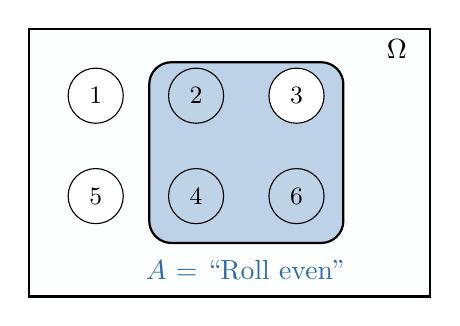
\begin{tikzpicture}[scale=0.85]
  % Rectangle (sample space) for die roll
  \draw[thick, fill=lightgray, fill opacity=0.2] (0,0) rectangle (6,4);
  \node at (5.5, 3.7) {$\Omega$};

  % Event A (even numbers) - highlighted region
  \draw[thick, fill=ocean, fill opacity=0.3, rounded corners=8pt] (1.8, 0.8) rectangle (4.7, 3.5);
  \node at (3.25, 0.4) {\textcolor{ocean}{$A$ = ``Roll even''}};

  % Individual outcomes
  \node[circle, draw, fill=white, minimum size=0.7cm] at (1, 3) {\small 1};
  \node[circle, draw, fill=ocean!30, minimum size=0.7cm] at (2.5, 3) {\small 2};
  \node[circle, draw, fill=white, minimum size=0.7cm] at (4, 3) {\small 3};
  \node[circle, draw, fill=ocean!30, minimum size=0.7cm] at (2.5, 1.5) {\small 4};
  \node[circle, draw, fill=white, minimum size=0.7cm] at (1, 1.5) {\small 5};
  \node[circle, draw, fill=ocean!30, minimum size=0.7cm] at (4, 1.5) {\small 6};
\end{tikzpicture}
\end{center}

\vspace{0.3em}

The event $A = \{2, 4, 6\}$ is a \highlight{subset} of $\Omega$: we write $A \subseteq \Omega$.

\vspace{0.3em}

\textbf{We assign probabilities to events}: $\Prob(A) = \Prob(\text{``Roll even''}) = 3/6 = 1/2$

\end{frame}

% ----------------------------------------------------------------------------

\begin{frame}
\frametitle{Sample Space vs.\ Events}
\framesubtitle{$A \subseteq \Omega$}

\vspace{0.3em}

\begin{center}
\begin{tabular}{p{5.5cm}|p{5.5cm}}
\textbf{Sample Space} $\Omega$ & \textbf{Event} $A$ \\
\midrule
\emph{All} possible outcomes & \emph{Some} possible outcomes \\
The ``universe'' & A subset of the universe \\
Fixed for a given experiment & Many different events possible \\
$\Prob(\Omega) = 1$ always & $0 \leq \Prob(A) \leq 1$ \\
\end{tabular}
\end{center}

\vspace{0.5em}

\textbf{Die roll example}:

\begin{itemize}
\item Sample space: $\Omega = \{1, 2, 3, 4, 5, 6\}$ --- all six faces
\item Event ``roll even'': $A = \{2, 4, 6\}$ --- three of the six faces
\item Event ``roll a six'': $B = \{6\}$ --- just one face
\end{itemize}

\end{frame}

% ----------------------------------------------------------------------------

\begin{frame}
\frametitle{Operations on Events}

\vspace{0.5em}

Events are sets, so we can combine them:

\vspace{1em}

\begin{tabular}{lll}
\textbf{Operation} & \textbf{Notation} & \textbf{Meaning} \\
\midrule
Union & $A \cup B$ & $A$ or $B$ (or both) \\
Intersection & $A \cap B$ & $A$ and $B$ \\
Complement & $A^c$ & not $A$ \\
Difference & $A \setminus B$ & $A$ but not $B$ \\
\end{tabular}

\vspace{1em}

\textbf{Example}: Die roll, $A = \{2, 4, 6\}$ (even), $B = \{1, 2, 3\}$ (small)

\begin{itemize}
\item $A \cap B = \{2\}$ (even AND small)
\item $A \cup B = \{1, 2, 3, 4, 6\}$ (even OR small)
\item $A^c = \{1, 3, 5\}$ (odd)
\end{itemize}

\end{frame}

% ----------------------------------------------------------------------------

\begin{frame}
\frametitle{Mutually Exclusive Events}

\vspace{0.3em}

Two events are \highlight{mutually exclusive} (or \emph{disjoint}) if they cannot both occur: $A \cap B = \emptyset$

\vspace{0.5em}

\begin{center}
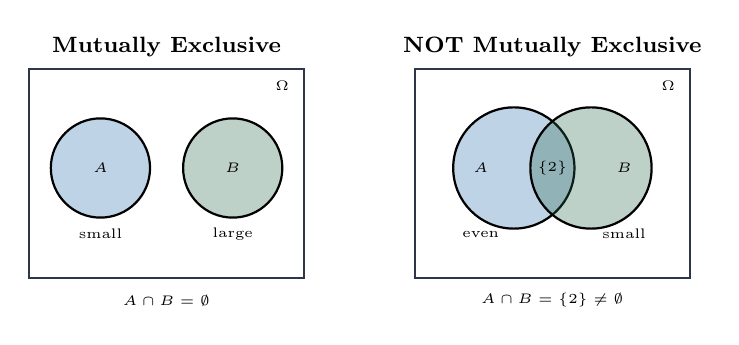
\begin{tikzpicture}[scale=0.7]
  % --- Mutually Exclusive (left) ---
  \node at (2.5, 4.2) {\footnotesize\textbf{Mutually Exclusive}};
  \draw[thick, color=charcoal] (0, 0) rectangle (5, 3.8);
  \node at (4.6, 3.5) {\tiny $\Omega$};

  % Circle A (small numbers)
  \draw[thick, fill=ocean, fill opacity=0.3] (1.3, 2) circle (0.9);
  \node at (1.3, 2) {\tiny $A$};
  \node at (1.3, 0.8) {\tiny small};

  % Circle B (large numbers) - separate
  \draw[thick, fill=forest, fill opacity=0.3] (3.7, 2) circle (0.9);
  \node at (3.7, 2) {\tiny $B$};
  \node at (3.7, 0.8) {\tiny large};

  \node at (2.5, -0.4) {\tiny $A \cap B = \emptyset$};

  % --- NOT Mutually Exclusive (right) ---
  \begin{scope}[xshift=7cm]
  \node at (2.5, 4.2) {\footnotesize\textbf{NOT Mutually Exclusive}};
  \draw[thick, color=charcoal] (0, 0) rectangle (5, 3.8);
  \node at (4.6, 3.5) {\tiny $\Omega$};

  % Circle A (even numbers)
  \draw[thick, fill=ocean, fill opacity=0.3] (1.8, 2) circle (1.1);
  \node at (1.2, 2) {\tiny $A$};
  \node at (1.2, 0.8) {\tiny even};

  % Circle B (small numbers) - overlapping
  \draw[thick, fill=forest, fill opacity=0.3] (3.2, 2) circle (1.1);
  \node at (3.8, 2) {\tiny $B$};
  \node at (3.8, 0.8) {\tiny small};

  % Intersection label
  \node at (2.5, 2) {\tiny $\{2\}$};

  \node at (2.5, -0.4) {\tiny $A \cap B = \{2\} \neq \emptyset$};
  \end{scope}
\end{tikzpicture}
\end{center}

\vspace{0.3em}

\textbf{Example}: Die roll --- $A = \{1,2,3\}$ (small), $B = \{4,5,6\}$ (large) are mutually exclusive.

\vspace{0.2em}

\deemph{Why does this matter? It simplifies probability calculations: $\Prob(A \cup B) = \Prob(A) + \Prob(B)$}

\end{frame}

% ----------------------------------------------------------------------------
% EVENT SPACES (SIGMA-ALGEBRAS)
% ----------------------------------------------------------------------------

\begin{frame}
\frametitle{Event Spaces}

\vspace{2em}

\begin{center}
\Huge
\textcolor{charcoal}{\textbf{Event Spaces}}
\end{center}

\vspace{1em}

\begin{center}
\large
\deemph{Which subsets can we assign probabilities to?}
\end{center}

\end{frame}

% ----------------------------------------------------------------------------

\begin{frame}
\frametitle{Election Night}
\framesubtitle{A story about asking questions}

\vspace{0.5em}

You're a campaign manager. It's election night. The race is tight.

\vspace{0.5em}

Three precincts remain uncounted: \textbf{North}, \textbf{South}, and \textbf{Central}.

\vspace{0.5em}

Exactly one of them will push your candidate over the top---the \emph{decisive} precinct.

\vspace{0.5em}

You're asking questions:

\begin{itemize}
\setlength{\itemsep}{4pt}
\item ``Will North be the one that decides it?''
\item ``Will it be one of our strongholds?''
\end{itemize}

\vspace{0.5em}

In probability language: $\Omega = \{\text{North}, \text{South}, \text{Central}\}$

\vspace{0.3em}

\deemph{Exactly one outcome will occur---whichever precinct decides the race.}

\end{frame}

% ----------------------------------------------------------------------------

\begin{frame}
\frametitle{Starting with the Bookends}
\framesubtitle{The certain and the impossible}

\vspace{0.5em}

Before asking specific questions, we need two things:

\vspace{0.8em}

\textbf{The certain event} $\Omega = \{\text{N}, \text{S}, \text{C}\}$:

``Some precinct will be decisive''---exactly one of them will decide the race. Probability = 1.

\vspace{0.8em}

\textbf{The impossible event} $\emptyset$:

``No precinct decides it''---can't happen; one of them must. Probability = 0.

\vspace{0.8em}

\textbf{Our event space so far}: $\mathcal{S} = \{\emptyset, \Omega\}$

\vspace{0.5em}

This is the \highlight{minimal event space}. We can only say ``some precinct decided it.'' We can't yet ask \emph{which} one.

\end{frame}

% ----------------------------------------------------------------------------

\begin{frame}
\frametitle{A Note on Notation}
\framesubtitle{The empty set symbol}

\vspace{1em}

This symbol: $\emptyset$

\vspace{1em}

It looks like the Greek letter theta ($\theta$), but it's not.

\vspace{1em}

It's the \highlight{empty set} symbol — a zero with a slash through it.

\vspace{1em}

\textbf{Pronunciation}: Just say ``the empty set.''

\vspace{1em}

\deemph{The symbol comes from Scandinavian languages (Ø), introduced by French mathematicians in the 1930s.}

\end{frame}

% ----------------------------------------------------------------------------

\begin{frame}
\frametitle{What Is the Empty Set?}
\framesubtitle{The impossible event}

\vspace{1em}

The empty set $\emptyset$ confuses people.

\vspace{1em}

What does ``no outcome'' mean?

\vspace{1em}

$\emptyset$ is \textbf{the event that contains no outcomes}.

\vspace{1em}

Since \emph{some} precinct must be decisive, $\emptyset$ cannot happen.

\vspace{1em}

It's the \highlight{impossible event}. Probability = 0.

\vspace{1em}

\deemph{But where does it come from? Why must every event space include it?}

\end{frame}

% ----------------------------------------------------------------------------

\begin{frame}
\frametitle{Why Must $\emptyset$ Be in Every Event Space?}
\framesubtitle{Complements again}

\vspace{1em}

Because $\emptyset$ is the complement of $\Omega$:

\vspace{1em}

\begin{itemize}
\setlength{\itemsep}{8pt}
\item $\Omega$ = ``something happens'' \quad (the certain event)
\item $\Omega^c$ = ``nothing happens'' = $\emptyset$ \quad (the impossible event)
\end{itemize}

\vspace{1em}

If $\Omega$ is in our event space, then $\emptyset$ must be too.

\vspace{1em}

\deemph{$\emptyset$ and $\Omega$ are the bookends---every event space contains both.}

\end{frame}

% ----------------------------------------------------------------------------

\begin{frame}
\frametitle{Adding a Question}
\framesubtitle{Building up the event space}

\vspace{0.5em}

Now you want to ask: ``Was North the decisive precinct?''

\vspace{0.5em}

That's the event $\{\text{North}\}$---the set containing just North.

\vspace{0.8em}

\textbf{Can we just add $\{\text{North}\}$ to our event space?}

\vspace{0.5em}

Not by itself. If we can ask ``Was it North?'' we must also be able to ask ``Was it \emph{not} North?''

\vspace{0.5em}

That's the complement: $\{\text{North}\}^c = \{\text{South}, \text{Central}\}$

\end{frame}

% ----------------------------------------------------------------------------

\begin{frame}
\frametitle{Adding a Question}
\framesubtitle{We must add both}

\vspace{0.8em}

\textbf{So we must add both the question and its opposite}:

\vspace{0.8em}

$\mathcal{S} = \{\emptyset, \{\text{North}\}, \{\text{South}, \text{Central}\}, \Omega\}$

\vspace{0.8em}

Now we can ask:
\begin{itemize}
\setlength{\itemsep}{3pt}
\item ``Was North decisive?'' \quad ($\{\text{North}\}$)
\item ``Was North \emph{not} decisive?'' \quad ($\{\text{South}, \text{Central}\}$)
\end{itemize}

\vspace{0.8em}

\textbf{How to read this}: $\{\text{South}, \text{Central}\}$ means ``the decisive precinct was \emph{either} South \emph{or} Central.'' The set lists the possibilities.

\end{frame}

% ----------------------------------------------------------------------------

\begin{frame}
\frametitle{Questions Come in Pairs}
\framesubtitle{The complement rule}

\vspace{0.5em}

This is \textbf{Property 2} of event spaces: \emph{closed under complements}.

\vspace{0.5em}

If you can ask a question, you can ask its opposite.

\vspace{0.8em}

\begin{center}
\begin{tabular}{ll}
\textbf{Question} & \textbf{Opposite} \\
\midrule
Was North decisive? & Was North \emph{not} decisive? \\
$\{\text{N}\}$ & $\{\text{S}, \text{C}\}$ \\
\midrule
Did some precinct decide it? & Did no precinct decide it? \\
$\Omega$ & $\emptyset$ \\
\end{tabular}
\end{center}

\vspace{0.8em}

\deemph{Every event in $\mathcal{S}$ must have its complement in $\mathcal{S}$ too.}

\end{frame}

% ----------------------------------------------------------------------------

\begin{frame}
\frametitle{Combining Questions}
\framesubtitle{Unions}

\vspace{0.3em}

What if you want to ask: ``Was it North \emph{or} South that decided it?''

\vspace{0.3em}

That's a union: $\{\text{North}\} \cup \{\text{South}\} = \{\text{North}, \text{South}\}$

\vspace{0.5em}

\textbf{Property 3}: If both $\{\text{N}\}$ and $\{\text{S}\}$ are in your event space, then $\{\text{N}, \text{S}\}$ must be too.

\vspace{0.5em}

And if $\{\text{N}, \text{S}\}$ is in, its complement $\{\text{C}\}$ must be in (Property 2).

\vspace{0.5em}

\textbf{The event space grows}:

Adding questions forces you to add their opposites and combinations.

\end{frame}

% ----------------------------------------------------------------------------

\begin{frame}
\frametitle{The Power Set}
\framesubtitle{The maximal event space}

\vspace{0.5em}

The \highlight{power set} $2^\Omega$ is the collection of \emph{all} subsets of $\Omega$.

\vspace{0.8em}

\textbf{How many subsets?} Each outcome is either \emph{in} or \emph{out} of a subset.

\vspace{0.3em}

With $n$ outcomes, that's $2 \times 2 \times \cdots \times 2 = 2^n$ possible subsets.

\vspace{0.8em}

\textbf{Our example}: $\Omega = \{\text{N}, \text{S}, \text{C}\}$ has 3 outcomes, so $2^3 = 8$ subsets.

\vspace{0.8em}

The power set is always a valid event space---it's ``maximal'' because it lets you ask \emph{any} question.

\end{frame}

% ----------------------------------------------------------------------------

\begin{frame}
\frametitle{The Power Set}
\framesubtitle{All 8 subsets, in complement pairs}

\vspace{0.5em}

For $\Omega = \{\text{N}, \text{S}, \text{C}\}$, the power set contains:

\vspace{0.5em}

\begin{center}
\begin{tabular}{cc}
\textbf{Event} & \textbf{Complement} \\
\midrule
$\emptyset$ & $\Omega = \{\text{N}, \text{S}, \text{C}\}$ \\
$\{\text{N}\}$ & $\{\text{S}, \text{C}\}$ \\
$\{\text{S}\}$ & $\{\text{N}, \text{C}\}$ \\
$\{\text{C}\}$ & $\{\text{N}, \text{S}\}$ \\
\end{tabular}
\end{center}

\vspace{0.5em}

That's 8 sets total (4 pairs).

\vspace{0.5em}

\deemph{Every element has a complement, and every possible question about which precinct was decisive can be asked.}

\end{frame}

% ----------------------------------------------------------------------------

\begin{frame}
\frametitle{Quick Notation Review}
\framesubtitle{Translating the story to symbols}

\vspace{0.3em}

Now let's formalize what we just built:

\vspace{0.5em}

\begin{tabular}{ll}
\textbf{Symbol} & \textbf{Meaning} \\
\midrule
$\Omega = \{\text{N}, \text{S}, \text{C}\}$ & Sample space: all possible outcomes \\
$\{\text{N}\}$ & A \highlight{singleton}: ``North was decisive'' \\
$\{\text{N}, \text{S}\}$ & ``North or South was decisive'' \\
$\emptyset$ & The empty set: the impossible event \\
$\mathcal{S}$ & Event space: the collection of questions we can ask \\
\end{tabular}

\vspace{0.5em}

\textbf{Key point}: $\mathcal{S}$ is a ``set of sets.'' Each element of $\mathcal{S}$ is a subset of $\Omega$.

\vspace{0.5em}

\textbf{Example}: $\mathcal{S} = \{\emptyset, \{\text{N}\}, \{\text{S},\text{C}\}, \Omega\}$ contains four sets (questions).

\end{frame}

% ----------------------------------------------------------------------------

\begin{frame}
\frametitle{Why Do We Need Event Spaces?}
\framesubtitle{A puzzle about infinite sample spaces}

\vspace{0.3em}

For finite sample spaces like $\Omega = \{1, 2, 3, 4, 5, 6\}$, we can assign probabilities to \emph{every} subset (all $2^6 = 64$ of them).

\vspace{0.5em}

\textbf{But what about infinite sample spaces?}

\vspace{0.3em}

If $\Omega = [0, 1]$ (all real numbers from 0 to 1), there are \emph{uncountably many} subsets. Some of these subsets are so pathological (i.e., so weird we can't assign probabilities to them) that we \emph{cannot} assign probabilities to them consistently.

\vspace{0.5em}

\textbf{The solution}: Don't try to assign probabilities to \emph{every} subset. Instead, specify a collection of ``well-behaved'' subsets---an \highlight{event space}---and only assign probabilities to those.

\vspace{0.5em}

\deemph{For finite sample spaces, the power set (all subsets) always works. The machinery of event spaces becomes essential for continuous random variables.}

\end{frame}

% ----------------------------------------------------------------------------

\begin{frame}
\frametitle{What Is an Event Space?}
\framesubtitle{The three properties}

\vspace{0.2em}

An \highlight{event space} (or $\sigma$-algebra) $\mathcal{S}$ on $\Omega$ is a \emph{collection of subsets} of $\Omega$. Think of $\mathcal{S}$ as a ``set of sets''---each element of $\mathcal{S}$ is itself a subset of $\Omega$. The notation $A \in \mathcal{S}$ means ``$A$ is one of the sets in $\mathcal{S}$.''

\vspace{0.2em}

A valid event space must satisfy three properties:

\vspace{0.2em}

\begin{enumerate}
\setlength{\itemsep}{0pt}
\item \textbf{Contains the sample space}: $\Omega \in \mathcal{S}$ \quad \deemph{($\Omega$ is one of the sets in $\mathcal{S}$)}

\item \textbf{Closed under complements}: If $A \in \mathcal{S}$, then $A^c \in \mathcal{S}$

\item \textbf{Closed under countable unions}: If $A_1, A_2, \ldots \in \mathcal{S}$, then $\bigcup_{i=1}^{\infty} A_i \in \mathcal{S}$
\end{enumerate}

\vspace{0.2em}

\highlight{Key point}: These properties ensure that when we combine events using ``or'', ``and'', or ``not'', we stay inside the event space.

\end{frame}

% ----------------------------------------------------------------------------

\begin{frame}
\frametitle{Common Patterns}
\framesubtitle{What to look for}

\vspace{0.5em}

\textbf{The trivial event space} $\mathcal{S} = \{\emptyset, \Omega\}$ \emph{always} works.

\vspace{0.8em}

\textbf{Event spaces come in complement pairs}:

If $A \in \mathcal{S}$, then $A^c$ must also be in $\mathcal{S}$.

So if you see $\{A\}$ without $\{B, C, D\}$ (its complement)? \textcolor{harvardcrimson}{Fails Property 2.}

\vspace{0.8em}

\textbf{Unions can create new sets}:

If $\{1\}$ and $\{2\}$ are both in $\mathcal{S}$, then $\{1,2\}$ must be too.

So if you see $\{1\}$ and $\{2\}$ but not $\{1,2\}$? \textcolor{harvardcrimson}{Fails Property 3.}

\vspace{0.8em}

\textbf{The power set} $2^\Omega$ (all subsets) is always valid---it's the ``maximal'' event space.

\end{frame}

% ----------------------------------------------------------------------------

\begin{frame}
\frametitle{Consequences of the Three Properties}
\framesubtitle{What follows automatically}

\vspace{0.2em}

From the three properties, we get additional facts \emph{for free}:

\vspace{0.3em}

\textbf{The empty set is always in $\mathcal{S}$}:
\begin{itemize}
\setlength{\itemsep}{0pt}
\item By (1): $\Omega \in \mathcal{S}$
\item By (2): $\Omega^c = \emptyset \in \mathcal{S}$ \checkmark
\end{itemize}

\vspace{0.2em}

\textbf{Closed under countable intersections} (De Morgan's laws):
\begin{itemize}
\setlength{\itemsep}{0pt}
\item If $A_1, A_2, \ldots \in \mathcal{S}$, then $\bigcap_{i=1}^{\infty} A_i \in \mathcal{S}$
\item Why? $\bigcap A_i = \left(\bigcup A_i^c\right)^c$, and we can take complements and unions
\end{itemize}

\vspace{0.2em}

\textbf{Closed under set difference}:
\begin{itemize}
\setlength{\itemsep}{0pt}
\item If $A, B \in \mathcal{S}$, then $A \setminus B = A \cap B^c \in \mathcal{S}$
\end{itemize}

\vspace{0.3em}

\deemph{The three properties give us a ``closed system'' for doing set operations.}

\end{frame}

% ----------------------------------------------------------------------------

\begin{frame}
\frametitle{Singletons}
\framesubtitle{Sets with exactly one element}

\vspace{0.3em}

A \highlight{singleton} is a set containing exactly one outcome.

\vspace{0.5em}

\textbf{Example}: If $\Omega = \{A, B, C\}$, the singletons are $\{A\}$, $\{B\}$, and $\{C\}$.

\vspace{0.5em}

\textbf{Why do singletons matter?}

\vspace{0.3em}

\begin{itemize}
\item Singletons represent \emph{elementary events}---specific outcomes
\item If every singleton is in $\mathcal{S}$, we can ask ``What's the probability of outcome $A$?''
\item The power set (all $2^n$ subsets) always includes all singletons
\item But smaller event spaces might not include all singletons!
\end{itemize}

\vspace{0.5em}

\textbf{Example}: $\mathcal{S} = \{\emptyset, \Omega\}$ is a valid event space, but it contains \emph{no} singletons. We can only ask about ``something happens'' or ``nothing happens''---not about specific outcomes.

\vspace{0.3em}

\deemph{PS1 asks about singletons on infinite sample spaces. Stay tuned.}

\end{frame}

% ----------------------------------------------------------------------------

\begin{frame}
\frametitle{Checking Event Spaces: The Method}
\framesubtitle{A systematic approach}

\vspace{0.5em}

\textbf{Given}: A sample space $\Omega$ and a collection of sets $\mathcal{S}$.

\vspace{0.5em}

\textbf{Question}: Is $\mathcal{S}$ an event space?

\vspace{1em}

\textbf{The checklist}:
\begin{enumerate}
\item \textbf{Property 1}: Is $\Omega \in \mathcal{S}$? \quad (Also check: is $\emptyset \in \mathcal{S}$?)

\vspace{0.5em}

\item \textbf{Property 2}: For \emph{every} set $A \in \mathcal{S}$, compute $A^c$ and check if $A^c \in \mathcal{S}$

\vspace{0.5em}

\item \textbf{Property 3}: For \emph{every pair} of sets in $\mathcal{S}$, compute their union and check if it's in $\mathcal{S}$
\end{enumerate}

\end{frame}

% ----------------------------------------------------------------------------

\begin{frame}
\frametitle{Key Skills for Checking Event Spaces}
\framesubtitle{What you need to be able to do}

\vspace{0.5em}

\textbf{Computing complements}:

If $\Omega = \{1,2,3\}$ and $A = \{1\}$, then $A^c = \{2,3\}$

\vspace{1em}

\textbf{Computing unions}:

$\{1\} \cup \{2,3\} = \{1,2,3\} = \Omega$

\vspace{1em}

\textbf{Being systematic}:

Check \emph{every} element, not just one or two. If even one complement or union is missing, the collection fails to be an event space.

\vspace{1em}

\deemph{Let's work through some examples on the board...}

\end{frame}

% ----------------------------------------------------------------------------

\begin{frame}
\frametitle{Let's Practice}
\framesubtitle{Board work}

\vspace{1em}

\begin{center}
\Large
\textcolor{forest}{\textbf{Examples on the board}}
\end{center}

\vspace{1em}

We'll work through checking whether specific collections are event spaces:

\vspace{0.5em}

\begin{enumerate}
\item A collection that \emph{is} an event space (verify all three properties)

\vspace{0.3em}

\item A collection that \emph{fails} to be an event space (find where it breaks)

\vspace{0.3em}

\item How to \emph{construct} a new event space by adding sets carefully
\end{enumerate}

\vspace{1em}

\deemph{These skills are directly relevant to Problem Set 1.}

\end{frame}

% ----------------------------------------------------------------------------

\begin{frame}
\frametitle{The Power Set}
\framesubtitle{The ``maximal'' event space}

\vspace{0.3em}

The \highlight{power set} $2^\Omega$ is the collection of \emph{all} subsets of $\Omega$.

\vspace{0.5em}

\textbf{Example}: If $\Omega = \{1, 2, 3\}$, then $2^\Omega$ has $2^3 = 8$ elements:

\vspace{0.2em}

\[
2^\Omega = \{\emptyset, \{1\}, \{2\}, \{3\}, \{1,2\}, \{1,3\}, \{2,3\}, \{1,2,3\}\}
\]

\vspace{0.5em}

\textbf{The power set is always a valid event space}:
\begin{itemize}
\item Property 1: $\Omega \in 2^\Omega$? \checkmark{} (every set is a subset of itself)
\item Property 2: Closed under complements? \checkmark{} ($A^c$ is always a subset of $\Omega$)
\item Property 3: Closed under unions? \checkmark{} (union of subsets is a subset)
\end{itemize}

\vspace{0.5em}

\deemph{For finite $\Omega$, we almost always use the power set. The distinction matters for infinite sample spaces.}

\end{frame}

% ----------------------------------------------------------------------------

\begin{frame}
\frametitle{Countable Infinite Sample Spaces}
\framesubtitle{A puzzle to think about}

\vspace{0.3em}

Consider a \highlight{countably infinite} sample space: $\Omega = \{A_1, A_2, A_3, \ldots\}$

\vspace{0.5em}

\textbf{Question}: Can we assign \emph{equal} probability to every singleton $\{A_i\}$?

\vspace{0.5em}

That is, can we have $\Prob(\{A_i\}) = p$ for the \emph{same} value $p$ for all $i$?

\vspace{0.5em}

\textbf{Hint}: Think about what the axioms tell us:
\begin{itemize}
\item What does \textbf{normalization} say about $\Prob(\Omega)$?
\item What does \textbf{countable additivity} say when events are mutually exclusive?
\item What are the possible values $p$ could take?
\end{itemize}

\vspace{0.5em}

\textbf{This is Problem Set 1, Question 2.} Use the axioms to work through the answer carefully.

\vspace{0.5em}

\deemph{The axioms of probability have real consequences---they constrain what's possible.}

\end{frame}

% ----------------------------------------------------------------------------

\begin{frame}
\frametitle{Event Spaces: Summary}
\framesubtitle{What you need to know for PS1}

\vspace{0.5em}

\textbf{An event space} $\mathcal{S}$ must satisfy three properties:
\begin{enumerate}
\setlength{\itemsep}{2pt}
\item Contains $\Omega$
\item Closed under complements
\item Closed under countable unions
\end{enumerate}

\vspace{1em}

\textbf{To verify}: Check each property explicitly---verify \emph{every} complement and \emph{every} union.

\vspace{1em}

\textbf{To construct}: Start with $\{\emptyset, \Omega\}$, add sets in complement pairs.

\vspace{1em}

\textbf{The power set} $2^\Omega$ is always a valid event space.

\end{frame}

% ----------------------------------------------------------------------------
% KOLMOGOROV AXIOMS
% ----------------------------------------------------------------------------

\begin{frame}
\frametitle{Kolmogorov Axioms}
\framesubtitle{The rules probability must follow}

\vspace{0.3em}

A \highlight{probability measure} $\Prob: \mathcal{S} \to [0, 1]$ satisfies three axioms:

\vspace{0.5em}

\begin{enumerate}
\item \textbf{Non-negativity}: $\Prob(A) \geq 0$ for all events $A$
\begin{itemize}
  \item[\deemph{$\rightarrow$}] \deemph{Probabilities can't be negative}
\end{itemize}
\vspace{0.3em}
\item \textbf{Normalization}: $\Prob(\Omega) = 1$
\begin{itemize}
  \item[\deemph{$\rightarrow$}] \deemph{Something must happen; probabilities sum to 1}
\end{itemize}
\vspace{0.3em}
\item \textbf{Countable additivity}: For mutually exclusive events $A_1, A_2, \ldots$:
\[
\Prob\left(\bigcup_{i=1}^{\infty} A_i\right) = \sum_{i=1}^{\infty} \Prob(A_i)
\]
\begin{itemize}
  \item[\deemph{$\rightarrow$}] \deemph{If events can't overlap, just add their probabilities}
\end{itemize}
\end{enumerate}

\vspace{1em}

\deemph{Everything else we'll derive follows from these three axioms.}

\end{frame}

% ----------------------------------------------------------------------------

\begin{frame}
\frametitle{Consequences of the Axioms}

\vspace{0.5em}

From the three axioms, we can prove:

\vspace{1em}

\begin{itemize}
\item \textbf{Complement rule}: $\Prob(A^c) = 1 - \Prob(A)$
\vspace{0.5em}
\item \textbf{Impossible event}: $\Prob(\emptyset) = 0$
\vspace{0.5em}
\item \textbf{Monotonicity}: If $A \subseteq B$, then $\Prob(A) \leq \Prob(B)$
\vspace{0.5em}
\item \textbf{Subtraction rule}: $\Prob(B \setminus A) = \Prob(B) - \Prob(A \cap B)$
\vspace{0.5em}
\item \textbf{Addition rule}: $\Prob(A \cup B) = \Prob(A) + \Prob(B) - \Prob(A \cap B)$
\end{itemize}

\vspace{1em}

\deemph{The addition rule corrects for double-counting the intersection.}

\end{frame}

% ----------------------------------------------------------------------------

\begin{frame}
\frametitle{Visualizing the Consequences}
\framesubtitle{Quick reference}

\vspace{0.3em}

\begin{center}
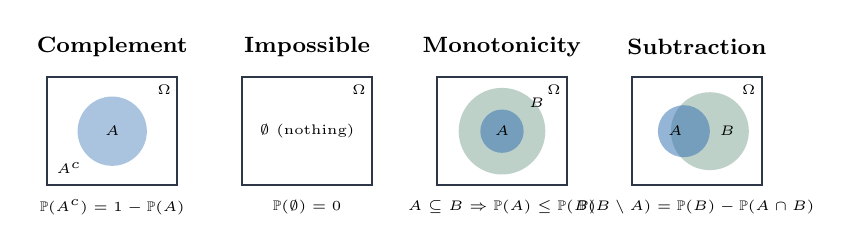
\begin{tikzpicture}[scale=0.55]
  % --- Complement Rule ---
  \node at (0, 3.2) {\footnotesize\textbf{Complement}};
  \draw[thick, color=charcoal] (-1.5, 0) rectangle (1.5, 2.5);
  \node at (1.2, 2.2) {\tiny $\Omega$};
  \fill[ocean, fill opacity=0.4] (0, 1.25) circle (0.8);
  \node at (0, 1.25) {\tiny $A$};
  \node at (-1, 0.4) {\tiny $A^c$};
  \node at (0, -0.5) {\tiny $\Prob(A^c) = 1 - \Prob(A)$};

  % --- Impossible Event ---
  \begin{scope}[xshift=4.5cm]
  \node at (0, 3.2) {\footnotesize\textbf{Impossible}};
  \draw[thick, color=charcoal] (-1.5, 0) rectangle (1.5, 2.5);
  \node at (1.2, 2.2) {\tiny $\Omega$};
  \node at (0, 1.25) {\tiny $\emptyset$ (nothing)};
  \node at (0, -0.5) {\tiny $\Prob(\emptyset) = 0$};
  \end{scope}

  % --- Monotonicity ---
  \begin{scope}[xshift=9cm]
  \node at (0, 3.2) {\footnotesize\textbf{Monotonicity}};
  \draw[thick, color=charcoal] (-1.5, 0) rectangle (1.5, 2.5);
  \node at (1.2, 2.2) {\tiny $\Omega$};
  \fill[forest, fill opacity=0.3] (0, 1.25) circle (1);
  \fill[ocean, fill opacity=0.5] (0, 1.25) circle (0.5);
  \node at (0, 1.25) {\tiny $A$};
  \node at (0.8, 1.9) {\tiny $B$};
  \node at (0, -0.5) {\tiny $A \subseteq B \Rightarrow \Prob(A) \leq \Prob(B)$};
  \end{scope}

  % --- Subtraction Rule ---
  \begin{scope}[xshift=13.5cm]
  \node at (0, 3.2) {\footnotesize\textbf{Subtraction}};
  \draw[thick, color=charcoal] (-1.5, 0) rectangle (1.5, 2.5);
  \node at (1.2, 2.2) {\tiny $\Omega$};
  \fill[forest, fill opacity=0.3] (0.3, 1.25) circle (0.9);
  \fill[ocean, fill opacity=0.5] (-0.3, 1.25) circle (0.6);
  \node at (-0.5, 1.25) {\tiny $A$};
  \node at (0.7, 1.25) {\tiny $B$};
  \node at (0, -0.5) {\tiny $\Prob(B \setminus A) = \Prob(B) - \Prob(A \cap B)$};
  \end{scope}
\end{tikzpicture}
\end{center}

\vspace{0.5em}

\deemph{Each follows from the three axioms. Proofs are in the readings.}

\end{frame}

% ----------------------------------------------------------------------------

\begin{frame}
\frametitle{The Addition Rule}
\framesubtitle{Visualizing inclusion-exclusion}

\vspace{1em}

\begin{center}
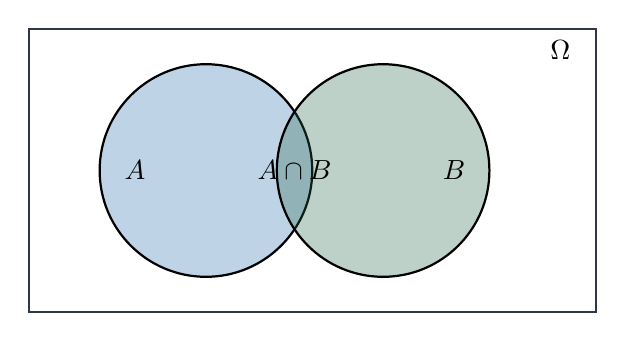
\begin{tikzpicture}[scale=0.9]
  % Rectangle (sample space)
  \draw[thick, color=charcoal] (0,0) rectangle (8,4);
  \node at (7.5, 3.7) {$\Omega$};

  % Circle A
  \draw[thick, fill=ocean, fill opacity=0.3] (2.5, 2) circle (1.5);
  \node at (1.5, 2) {$A$};

  % Circle B
  \draw[thick, fill=forest, fill opacity=0.3] (5, 2) circle (1.5);
  \node at (6, 2) {$B$};

  % Intersection label
  \node at (3.75, 2) {$A \cap B$};
\end{tikzpicture}
\end{center}

\vspace{0.5em}

\[
\Prob(A \cup B) = \Prob(A) + \Prob(B) - \Prob(A \cap B)
\]

\vspace{0.5em}

\deemph{If we add $\Prob(A)$ and $\Prob(B)$, we count the intersection twice.}

\end{frame}

% ----------------------------------------------------------------------------
% PART II: CONDITIONAL PROBABILITY
% ----------------------------------------------------------------------------

\begin{frame}
\frametitle{Part II}

\vspace{2em}

\begin{center}
\Huge
\textcolor{charcoal}{\textbf{Conditional Probability}}
\end{center}

\vspace{1em}

\begin{center}
\large
\deemph{Updating beliefs with new information}
\end{center}

\end{frame}

% ----------------------------------------------------------------------------

\begin{frame}
\frametitle{Conditional Probability}
\framesubtitle{The key definition}

\vspace{0.5em}

The \highlight{conditional probability} of $A$ given $B$ is:

\vspace{0.5em}

\[
\Prob(A \mid B) = \frac{\Prob(A \cap B)}{\Prob(B)} \qquad \text{provided } \Prob(B) > 0
\]

\vspace{1em}

\textbf{Interpretation}: The probability of $A$, \emph{given that we know $B$ occurred}.

\vspace{1em}

\deemph{We ``zoom in'' on the world where $B$ happened and ask: how much of that world is $A$?}

\end{frame}

% ----------------------------------------------------------------------------

\begin{frame}
\frametitle{Conditional Probability}
\framesubtitle{Visual intuition}

\vspace{0.5em}

\begin{center}
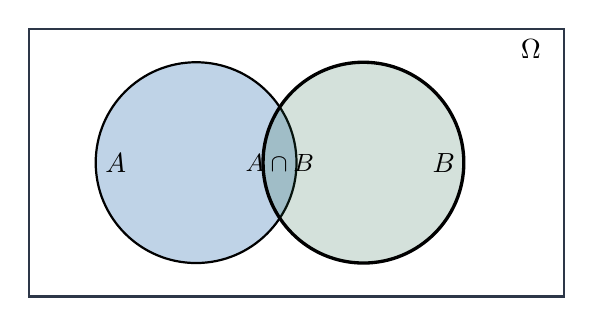
\begin{tikzpicture}[scale=0.85]
  % Rectangle (sample space)
  \draw[thick, color=charcoal] (0,0) rectangle (8,4);
  \node at (7.5, 3.7) {$\Omega$};

  % Circle A
  \draw[thick, fill=ocean, fill opacity=0.3] (2.5, 2) circle (1.5);
  \node at (1.3, 2) {$A$};

  % Circle B - highlighted as the new sample space
  \draw[very thick, fill=forest, fill opacity=0.2] (5, 2) circle (1.5);
  \node at (6.2, 2) {$B$};

  % Intersection
  \node at (3.75, 2) {\small $A \cap B$};
\end{tikzpicture}
\end{center}

\vspace{0.5em}

\[
\Prob(A \mid B) = \frac{\text{Probability of being in both } A \text{ and } B}{\text{Probability of being in } B}
\]

\vspace{0.5em}

\deemph{Given that we're in $B$, what fraction is also in $A$?}

\end{frame}

% ----------------------------------------------------------------------------

\begin{frame}
\frametitle{Example: Two Dice}

\vspace{0.5em}

Roll two fair dice. What is $\Prob(\text{sum} = 8 \mid \text{first die} = 3)$?

\vspace{1em}

\textbf{Solution}:
\begin{itemize}
\item Let $A = \{\text{sum} = 8\}$ and $B = \{\text{first die} = 3\}$
\vspace{0.3em}
\item $\Prob(B) = 6/36 = 1/6$ (six outcomes where first die is 3)
\vspace{0.3em}
\item $A \cap B = \{(3, 5)\}$ (only way to get sum 8 with first die 3)
\vspace{0.3em}
\item $\Prob(A \cap B) = 1/36$
\end{itemize}

\vspace{0.5em}

\[
\Prob(A \mid B) = \frac{1/36}{1/6} = \frac{1}{6}
\]

\vspace{0.5em}

\deemph{Compare to $\Prob(\text{sum} = 8) = 5/36 \approx 0.14$. Knowing the first die changes things!}

\end{frame}

% ----------------------------------------------------------------------------

\begin{frame}
\frametitle{The Multiplicative Law}

\vspace{0.3em}

Rearranging the definition of conditional probability:
\[
\Prob(A \cap B) = \Prob(A \mid B) \cdot \Prob(B)
\]

Or equivalently:
\[
\Prob(A \cap B) = \Prob(B \mid A) \cdot \Prob(A)
\]

\vspace{0.5em}

\textbf{The chain rule} (for three events):
\[
\Prob(A \cap B \cap C) = \Prob(A) \cdot \Prob(B \mid A) \cdot \Prob(C \mid A \cap B)
\]

\end{frame}

% ----------------------------------------------------------------------------

\begin{frame}
\frametitle{Visualizing the Multiplicative Law}
\framesubtitle{Two ways to compute $\Prob(A \cap B)$}

\vspace{0.3em}

\begin{center}
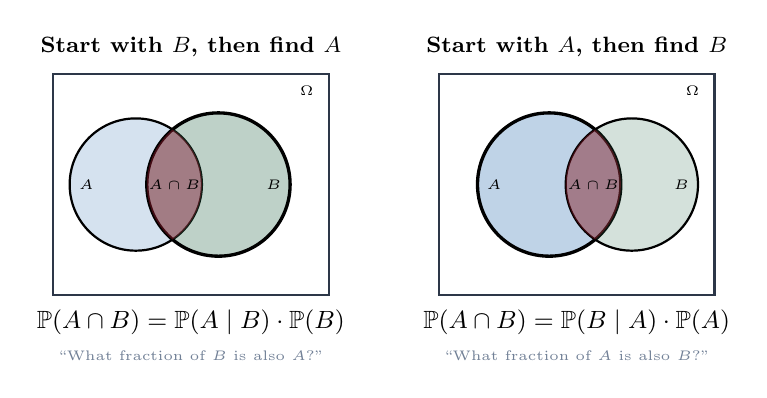
\begin{tikzpicture}[scale=0.7]
  % --- Left diagram: Condition on B ---
  \node at (2.5, 4.5) {\footnotesize\textbf{Start with $B$, then find $A$}};
  \draw[thick, color=charcoal] (0, 0) rectangle (5, 4);
  \node at (4.6, 3.7) {\tiny $\Omega$};

  % Circle A
  \draw[thick, fill=ocean, fill opacity=0.2] (1.5, 2) circle (1.2);
  \node at (0.6, 2) {\tiny $A$};

  % Circle B - emphasized
  \draw[very thick, fill=forest, fill opacity=0.3] (3, 2) circle (1.3);
  \node at (4, 2) {\tiny $B$};

  % Intersection - darkened
  \begin{scope}
    \clip (1.5, 2) circle (1.2);
    \fill[harvardcrimson, fill opacity=0.4] (3, 2) circle (1.3);
  \end{scope}

  \node at (2.2, 2) {\tiny $A \cap B$};

  % Formula below
  \node at (2.5, -0.5) {\small $\Prob(A \cap B) = \Prob(A \mid B) \cdot \Prob(B)$};
  \node at (2.5, -1.1) {\tiny\deemph{``What fraction of $B$ is also $A$?''}};

  % --- Right diagram: Condition on A ---
  \begin{scope}[xshift=7cm]
  \node at (2.5, 4.5) {\footnotesize\textbf{Start with $A$, then find $B$}};
  \draw[thick, color=charcoal] (0, 0) rectangle (5, 4);
  \node at (4.6, 3.7) {\tiny $\Omega$};

  % Circle A - emphasized
  \draw[very thick, fill=ocean, fill opacity=0.3] (2, 2) circle (1.3);
  \node at (1, 2) {\tiny $A$};

  % Circle B
  \draw[thick, fill=forest, fill opacity=0.2] (3.5, 2) circle (1.2);
  \node at (4.4, 2) {\tiny $B$};

  % Intersection - darkened
  \begin{scope}
    \clip (2, 2) circle (1.3);
    \fill[harvardcrimson, fill opacity=0.4] (3.5, 2) circle (1.2);
  \end{scope}

  \node at (2.8, 2) {\tiny $A \cap B$};

  % Formula below
  \node at (2.5, -0.5) {\small $\Prob(A \cap B) = \Prob(B \mid A) \cdot \Prob(A)$};
  \node at (2.5, -1.1) {\tiny\deemph{``What fraction of $A$ is also $B$?''}};
  \end{scope}
\end{tikzpicture}
\end{center}

\vspace{0.3em}

\highlight{Key insight}: The intersection $A \cap B$ is the same region either way---we're just computing its probability through different ``doors.''

\end{frame}

% ----------------------------------------------------------------------------

\begin{frame}
\frametitle{Visualizing the Chain Rule}
\framesubtitle{$\Prob(A \cap B \cap C) = \Prob(A) \cdot \Prob(B \mid A) \cdot \Prob(C \mid A \cap B)$}

\vspace{0.2em}

\begin{center}
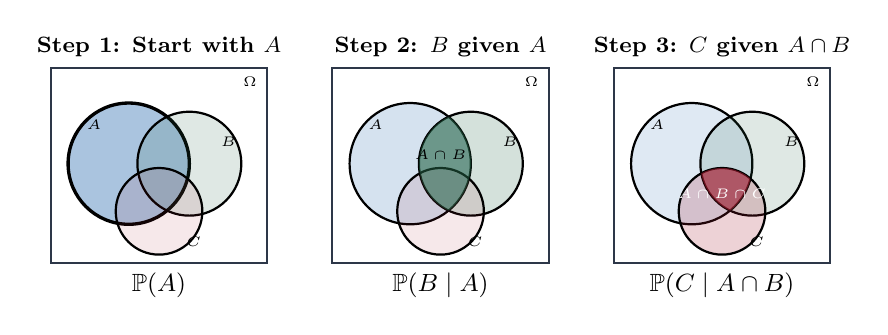
\begin{tikzpicture}[scale=0.55]
  % --- Step 1: Start with A ---
  \node at (2.5, 5) {\footnotesize\textbf{Step 1: Start with $A$}};
  \draw[thick, color=charcoal] (0, 0) rectangle (5, 4.5);
  \node at (4.6, 4.2) {\tiny $\Omega$};

  % All three circles shown lightly
  \draw[very thick, fill=ocean, fill opacity=0.4] (1.8, 2.3) circle (1.4);
  \draw[thick, fill=forest, fill opacity=0.15] (3.2, 2.3) circle (1.2);
  \draw[thick, fill=harvardcrimson, fill opacity=0.1] (2.5, 1.2) circle (1);

  \node at (1, 3.2) {\tiny $A$};
  \node at (4.1, 2.8) {\tiny $B$};
  \node at (3.3, 0.5) {\tiny $C$};

  \node at (2.5, -0.5) {\small $\Prob(A)$};

  % --- Step 2: Then B given A ---
  \begin{scope}[xshift=6.5cm]
  \node at (2.5, 5) {\footnotesize\textbf{Step 2: $B$ given $A$}};
  \draw[thick, color=charcoal] (0, 0) rectangle (5, 4.5);
  \node at (4.6, 4.2) {\tiny $\Omega$};

  % A shown, B|A intersection highlighted
  \draw[thick, fill=ocean, fill opacity=0.2] (1.8, 2.3) circle (1.4);
  \draw[thick, fill=forest, fill opacity=0.2] (3.2, 2.3) circle (1.2);
  \draw[thick, fill=harvardcrimson, fill opacity=0.1] (2.5, 1.2) circle (1);

  % Highlight A ∩ B
  \begin{scope}
    \clip (1.8, 2.3) circle (1.4);
    \fill[forest, fill opacity=0.5] (3.2, 2.3) circle (1.2);
  \end{scope}

  \node at (1, 3.2) {\tiny $A$};
  \node at (4.1, 2.8) {\tiny $B$};
  \node at (3.3, 0.5) {\tiny $C$};
  \node at (2.5, 2.5) {\tiny $A \cap B$};

  \node at (2.5, -0.5) {\small $\Prob(B \mid A)$};
  \end{scope}

  % --- Step 3: Then C given A ∩ B ---
  \begin{scope}[xshift=13cm]
  \node at (2.5, 5) {\footnotesize\textbf{Step 3: $C$ given $A \cap B$}};
  \draw[thick, color=charcoal] (0, 0) rectangle (5, 4.5);
  \node at (4.6, 4.2) {\tiny $\Omega$};

  % All circles shown lightly
  \draw[thick, fill=ocean, fill opacity=0.15] (1.8, 2.3) circle (1.4);
  \draw[thick, fill=forest, fill opacity=0.15] (3.2, 2.3) circle (1.2);
  \draw[thick, fill=harvardcrimson, fill opacity=0.2] (2.5, 1.2) circle (1);

  % Highlight A ∩ B ∩ C (the final target)
  \begin{scope}
    \clip (1.8, 2.3) circle (1.4);
    \clip (3.2, 2.3) circle (1.2);
    \fill[harvardcrimson, fill opacity=0.6] (2.5, 1.2) circle (1);
  \end{scope}

  \node at (1, 3.2) {\tiny $A$};
  \node at (4.1, 2.8) {\tiny $B$};
  \node at (3.3, 0.5) {\tiny $C$};
  \node at (2.5, 1.6) {\tiny\textcolor{white}{$A \cap B \cap C$}};

  \node at (2.5, -0.5) {\small $\Prob(C \mid A \cap B)$};
  \end{scope}
\end{tikzpicture}
\end{center}

\vspace{0.3em}

\highlight{Intuition}: Keep ``zooming in.'' First restrict to $A$, then to $A \cap B$, then ask what fraction is also in $C$.

\vspace{0.2em}

\deemph{Each step narrows the universe; each conditional probability asks ``what fraction of where we are is also in the next set?''}

\end{frame}

% ----------------------------------------------------------------------------
% PART III: INDEPENDENCE
% ----------------------------------------------------------------------------

\begin{frame}
\frametitle{Part III}

\vspace{2em}

\begin{center}
\Huge
\textcolor{charcoal}{\textbf{Independence}}
\end{center}

\vspace{1em}

\begin{center}
\large
\deemph{When knowing one thing tells you nothing about another}
\end{center}

\end{frame}

% ----------------------------------------------------------------------------

\begin{frame}
\frametitle{Independence of Events}
\framesubtitle{Definition}

\vspace{0.3em}

Events $A$ and $B$ are \highlight{independent} if:
\[
\Prob(A \cap B) = \Prob(A) \cdot \Prob(B)
\]

\textbf{Equivalent statement} (when $\Prob(B) > 0$):
\[
\Prob(A \mid B) = \Prob(A)
\]

\deemph{Knowing $B$ occurred doesn't change the probability of $A$.}

\vspace{0.3em}

\highlight{Independence means information is irrelevant.} Learning $B$ happened gives you no information about whether $A$ happened.

\vspace{0.3em}

\textbf{Notation}: $A \indep B$ means ``$A$ is independent of $B$''

\end{frame}

% ----------------------------------------------------------------------------

\begin{frame}
\frametitle{Independence vs.\ Mutual Exclusivity}
\framesubtitle{These are NOT the same thing!}

\vspace{0.5em}

\textbf{Mutually exclusive}: $A \cap B = \emptyset$ (can't both happen)

\vspace{0.3em}

\textbf{Independent}: $\Prob(A \cap B) = \Prob(A)\Prob(B)$ (knowing one doesn't affect the other)

\vspace{1em}

\textbf{In fact, they're almost opposites!}

\vspace{0.5em}

If $A$ and $B$ are mutually exclusive with $\Prob(A) > 0$ and $\Prob(B) > 0$:

\[
\Prob(A \mid B) = \frac{\Prob(A \cap B)}{\Prob(B)} = \frac{0}{\Prob(B)} = 0 \neq \Prob(A)
\]

\vspace{0.5em}

So mutually exclusive events are \textbf{dependent} (strongly so!).

\vspace{0.5em}

\deemph{If I know $B$ happened, I know $A$ didn't happen.}

\end{frame}

% ----------------------------------------------------------------------------

\begin{frame}
\frametitle{Example: Coin Flips}

Flip a fair coin twice. Let $A = \{\text{first flip is Heads}\}$ and $B = \{\text{second flip is Heads}\}$.

\vspace{0.5em}

Are $A$ and $B$ independent?

\vspace{0.5em}

\textbf{Check}:
\begin{itemize}
\item $\Prob(A) = 1/2$, \quad $\Prob(B) = 1/2$
\item $\Prob(A \cap B) = \Prob(\{HH\}) = 1/4$
\item $\Prob(A) \cdot \Prob(B) = (1/2)(1/2) = 1/4$ \checkmark
\end{itemize}

\vspace{0.5em}

\highlight{Yes}, they are independent. \deemph{The outcome of one flip doesn't affect the other.}

\end{frame}

% ----------------------------------------------------------------------------

\begin{frame}
\frametitle{Example: Drawing Cards}

\vspace{0.3em}

Draw two cards from a deck \textbf{without replacement}. Let:
\begin{itemize}
\item $A = \{\text{first card is an Ace}\}$, \quad $B = \{\text{second card is an Ace}\}$
\end{itemize}

Are $A$ and $B$ independent?

\vspace{0.3em}

\textbf{Check}:
\begin{itemize}
\item $\Prob(A) = 4/52$
\item $\Prob(B \mid A) = 3/51$ (if first was Ace, only 3 Aces left in 51 cards)
\item $\Prob(B \mid A^c) = 4/51$ (if first wasn't Ace, still 4 Aces in 51 cards)
\end{itemize}

\vspace{0.3em}

Since $\Prob(B \mid A) \neq \Prob(B \mid A^c)$, knowing $A$ changes $\Prob(B)$.

\vspace{0.3em}

\highlight{No}, they are \textbf{not} independent.

\end{frame}

% ----------------------------------------------------------------------------
% PART IV: BAYES' RULE
% ----------------------------------------------------------------------------

\begin{frame}
\frametitle{Part IV}

\vspace{2em}

\begin{center}
\Huge
\textcolor{charcoal}{\textbf{Bayes' Rule}}
\end{center}

\vspace{1em}

\begin{center}
\large
\deemph{Reversing conditional probabilities}
\end{center}

\end{frame}

% ----------------------------------------------------------------------------

\begin{frame}
\frametitle{The Reverend Thomas Bayes (1701--1761)}
\framesubtitle{A thought experiment with billiard balls}

\vspace{0.3em}

Thomas Bayes was an English Presbyterian minister and amateur mathematician. His famous essay was published posthumously in 1763 by his friend Richard Price.

\vspace{0.5em}

\textbf{Bayes' thought experiment}: Imagine a billiard table. A ball is rolled and comes to rest somewhere---you don't see where. Then more balls are rolled, and you're told whether each lands to the left or right of the first ball.

\vspace{0.5em}

\textbf{The question}: Given this evidence, what can you infer about where the first ball is?

\vspace{0.5em}

\highlight{Key insight}: Each new observation lets us \emph{update} our beliefs about the unknown quantity. We start with uncertainty (a ``prior''), observe evidence, and arrive at refined beliefs (a ``posterior'').

\vspace{0.3em}

\deemph{This is the logic of Bayesian inference: prior $\times$ likelihood $\rightarrow$ posterior.}

\end{frame}

% ----------------------------------------------------------------------------

\begin{frame}
\frametitle{A Controversial Idea}
\framesubtitle{The frequentist-Bayesian debate}

Bayes' approach was \highlight{controversial} for over 200 years. Why?

\vspace{0.2em}

\textbf{Frequentist objection}: Probability should describe long-run frequencies of \emph{repeatable} events. ``There's a 70\% probability the ball is in the left half'' seemed unscientific---the ball is either there or it isn't!

\vspace{0.2em}

\textbf{Bayesian response}: Probability describes our \emph{uncertainty}, not physical randomness. It's sensible to have beliefs about fixed but unknown quantities.

\vspace{0.2em}

\textbf{Historical irony}: Statisticians dismissed Bayesian methods as ``subjective'' well into the 20th century. Yet Bayesian reasoning proved essential in:
\begin{itemize}
\setlength{\itemsep}{0pt}
\item Breaking the Nazi Enigma code (1940s)
\item Finding lost submarines and aircraft (1960s--today)
\item Modern machine learning and AI
\end{itemize}

\vspace{-0.5em}
\deemph{Today, most statisticians use both approaches as tools for different problems.}

\end{frame}

% ----------------------------------------------------------------------------

\begin{frame}
\frametitle{Bayes' Rule in History}
\framesubtitle{From codebreaking to search and rescue}

\vspace{0.3em}

\textbf{Alan Turing (1940s)}: Used sequential Bayesian updating to crack the Nazi Enigma code at Bletchley Park. Each piece of intercepted message updated beliefs about machine settings. \deemph{He called it ``banburismus'' after the town of Banbury, where the paper strips were made.}

\vspace{0.5em}

\textbf{Search Theory (1960s--today)}:
\begin{itemize}
\item \textbf{USS \emph{Scorpion} (1968)}: Navy used Bayesian search to find the lost submarine
\item \textbf{Air France 447 (2009)}: After two years of failed searches, Bayesian methods found the wreckage
\item \textbf{Steve Fossett (2007)}: Updated probability maps based on search patterns
\item \textbf{MH370 (2014)}: Bayesian analysis of satellite data guided the search
\end{itemize}

\vspace{0.3em}

\highlight{The logic}: Start with prior beliefs about location. Each failed search in an area \emph{lowers} the probability there and \emph{raises} it elsewhere.

\end{frame}

% ----------------------------------------------------------------------------

\begin{frame}
\frametitle{Motivation: Strategic Thinking Under Uncertainty}

\vspace{0.5em}

\textbf{Example}: You're playing poker, and the person in front of you raises.

\vspace{0.5em}

What's your best response?

\vspace{0.5em}

\begin{itemize}
\item It depends on what you \emph{learned} from that raise
\item And what cards you're holding
\end{itemize}

\vspace{1em}

This requires us to \highlight{update our beliefs} based on new information.

\vspace{1em}

We need to calculate conditional probabilities---but often we know them ``backwards.''

\end{frame}

% ----------------------------------------------------------------------------

\begin{frame}
\frametitle{A Hiring Problem}
\framesubtitle{The firm's dilemma}

\vspace{0.3em}

You're a firm deciding whether to hire a job applicant.

\vspace{0.3em}

\textbf{The problem}: Workers come in two types:
\begin{itemize}
\setlength{\itemsep}{2pt}
\item \textbf{High type} --- productive, will make your firm money
\item \textbf{Low type} --- unproductive, will cost you money
\end{itemize}

\vspace{0.3em}

Unfortunately, you \emph{can't directly observe} which type they are. But you \emph{can} observe whether they have an MBA.

\vspace{0.3em}

\textbf{Your question}: Given that this applicant has an MBA, what's the probability they're a high type?

\vspace{0.5em}

\deemph{This problem combines three Nobel Prizes: signaling (Spence), types (Harsanyi), and subgame perfect Bayesian Nash equilibrium (Selten). We'll just do the Bayes part.}

\end{frame}

% ----------------------------------------------------------------------------

\begin{frame}
\frametitle{Setting Up the Problem}
\framesubtitle{Events and notation}

\vspace{0.8em}

Let's define two events:
\begin{itemize}
\setlength{\itemsep}{6pt}
\item $H$ = ``Worker is high type'' (productive)
\item $MBA$ = ``Worker has an MBA''
\end{itemize}

\vspace{0.8em}

The firm wants to know: $\Prob(H \mid MBA)$

\vspace{0.5em}

\deemph{``What's the probability this worker is productive, \emph{given} that they have an MBA?''}

\vspace{0.8em}

The MBA is something economists call a \highlight{signal}---an observable action that might reveal hidden information about type.

\end{frame}

% ----------------------------------------------------------------------------

\begin{frame}
\frametitle{What Can the Firm Observe?}
\framesubtitle{The available data}

\vspace{0.5em}

The firm can observe:

\vspace{0.5em}

\begin{itemize}
\setlength{\itemsep}{6pt}
\item $\Prob(H)$ --- the base rate of high types in the population
\item $\Prob(MBA)$ --- the fraction of applicants with MBAs
\item $\Prob(MBA \mid H)$ --- among high types, what fraction get MBAs?
\end{itemize}

\vspace{0.8em}

But the firm wants $\Prob(H \mid MBA)$ --- the probability of high type \emph{given} they see the signal.

\vspace{0.8em}

\textbf{The problem}: We know $\Prob(MBA \mid H)$, but we want $\Prob(H \mid MBA)$.

\vspace{0.5em}

We need to ``flip'' the conditional. That's what Bayes' Rule does.

\end{frame}

% ----------------------------------------------------------------------------

\begin{frame}
\frametitle{Deriving Bayes' Rule}
\framesubtitle{Step by step from definitions}

Let $A$ and $B$ be two events. We want $\Prob(A \mid B)$.

\vspace{0.3em}

\textbf{Start with the definition of conditional probability:}
\[
\Prob(A \mid B) = \frac{\Prob(A \cap B)}{\Prob(B)} \quad \Longrightarrow \quad \Prob(A \cap B) = \Prob(A \mid B) \cdot \Prob(B)
\]

\textbf{Similarly:}
\[
\Prob(B \mid A) = \frac{\Prob(B \cap A)}{\Prob(A)} \quad \Longrightarrow \quad \Prob(B \cap A) = \Prob(B \mid A) \cdot \Prob(A)
\]

\end{frame}

% ----------------------------------------------------------------------------

\begin{frame}
\frametitle{Deriving Bayes' Rule}
\framesubtitle{The key insight}

\vspace{0.3em}

Since $\Prob(A \cap B) = \Prob(B \cap A)$:
\[
\Prob(A \mid B) \cdot \Prob(B) = \Prob(B \mid A) \cdot \Prob(A)
\]

\textbf{Solve for $\Prob(A \mid B)$:}

\begin{center}
\Large
\textcolor{forest}{
$\Prob(A \mid B) = \dfrac{\Prob(B \mid A) \cdot \Prob(A)}{\Prob(B)}$
}
\end{center}

\vspace{0.5em}

This is \highlight{Bayes' Rule} (naive form).

\deemph{It lets us ``flip'' conditional probabilities: from $\Prob(B \mid A)$ to $\Prob(A \mid B)$.}

\end{frame}

% ----------------------------------------------------------------------------

\begin{frame}
\frametitle{Visualizing Bayes' Rule}
\framesubtitle{The tree diagram: forward vs.\ backward}

\begin{center}
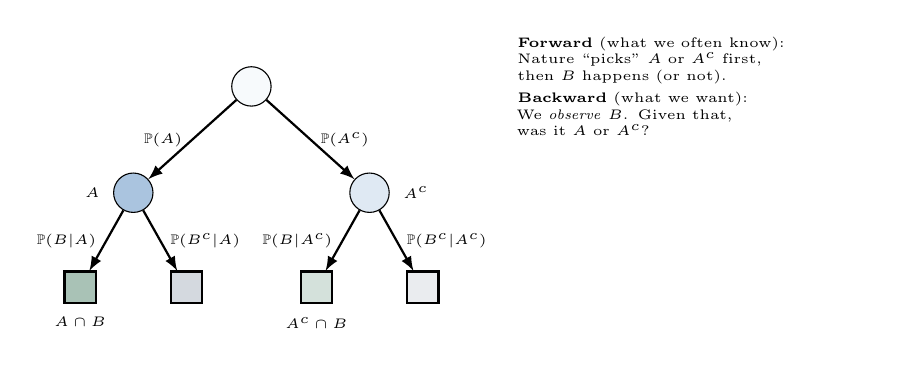
\begin{tikzpicture}[
  level 1/.style={sibling distance=4cm, level distance=1.8cm},
  level 2/.style={sibling distance=1.8cm, level distance=1.6cm},
  every node/.style={font=\footnotesize},
  edge from parent/.style={draw, thick, -latex},
  scale=0.75
]

% Root
\node[circle, draw, fill=lightgray, minimum size=0.5cm] (root) {}
  child {
    node[circle, draw, fill=ocean!40, minimum size=0.5cm] (A) {}
    child {
      node[rectangle, draw, fill=forest!40, minimum size=0.4cm] (AB) {}
      edge from parent node[left, font=\tiny] {$\Prob(B|A)$}
    }
    child {
      node[rectangle, draw, fill=warmgray!30, minimum size=0.4cm] (ABc) {}
      edge from parent node[right, font=\tiny] {$\Prob(B^c|A)$}
    }
    edge from parent node[left, font=\tiny] {$\Prob(A)$}
  }
  child {
    node[circle, draw, fill=ocean!15, minimum size=0.5cm] (Ac) {}
    child {
      node[rectangle, draw, fill=forest!20, minimum size=0.4cm] (AcB) {}
      edge from parent node[left, font=\tiny] {$\Prob(B|A^c)$}
    }
    child {
      node[rectangle, draw, fill=warmgray!15, minimum size=0.4cm] (AcBc) {}
      edge from parent node[right, font=\tiny] {$\Prob(B^c|A^c)$}
    }
    edge from parent node[right, font=\tiny] {$\Prob(A^c)$}
  };

% Labels
\node[left=0.05cm of A, font=\tiny] {$A$};
\node[right=0.05cm of Ac, font=\tiny] {$A^c$};
\node[below=0.05cm of AB, font=\tiny] {$A \cap B$};
\node[below=0.05cm of AcB, font=\tiny] {$A^c \cap B$};

% Annotations
\node[right=3cm of root, text width=4.5cm, font=\tiny] {
\textbf{Forward} (what we often know):\\
Nature ``picks'' $A$ or $A^c$ first,\\
then $B$ happens (or not).\\[0.3em]
\textbf{Backward} (what we want):\\
We \emph{observe} $B$. Given that,\\
was it $A$ or $A^c$?
};

\end{tikzpicture}
\end{center}

\textbf{Bayes' Rule}: Of all the ways to reach $B$, what fraction came through $A$?

\vspace{-0.3em}

\[
\Prob(A \mid B) = \frac{\Prob(A \cap B)}{\Prob(A \cap B) + \Prob(A^c \cap B)} = \frac{\text{green path through } A}{\text{all green paths}}
\]

\end{frame}

% ----------------------------------------------------------------------------

\begin{frame}
\frametitle{The Law of Total Probability}
\framesubtitle{A consequence of the additivity axiom}

\vspace{0.3em}

\textbf{Observation}: We can decompose $B$ using a \highlight{partition} of $\Omega$:
$B = (B \cap A) \cup (B \cap A^c)$

\vspace{0.2em}

A partition is a collection of mutually exclusive, exhaustive ``bins.'' Here $\{A, A^c\}$ partitions $\Omega$.

\vspace{0.2em}

These pieces are mutually exclusive, so by the \textbf{additivity axiom}:
\[
\Prob(B) = \Prob(B \cap A) + \Prob(B \cap A^c)
\]

\textbf{Apply the multiplicative law}:
\[
\Prob(B) = \Prob(B \mid A) \cdot \Prob(A) + \Prob(B \mid A^c) \cdot \Prob(A^c)
\]

\deemph{The unconditional probability is a weighted average of conditional probabilities.}

\highlight{This gives us what we need for Bayes' denominator.}

\end{frame}

% ----------------------------------------------------------------------------

\begin{frame}
\frametitle{Bayes' Rule: Full Form}

\vspace{0.5em}

Substituting the Law of Total Probability into Bayes' Rule:

\vspace{1em}

\begin{center}
\Large
\textcolor{forest}{
$\Prob(A \mid B) = \dfrac{\Prob(B \mid A) \cdot \Prob(A)}{\Prob(B \mid A) \cdot \Prob(A) + \Prob(B \mid A^c) \cdot \Prob(A^c)}$
}
\end{center}

\vspace{1.5em}

\textbf{Terminology}:
\begin{itemize}
\item $\Prob(A)$: \highlight{Prior} --- belief before seeing $B$
\item $\Prob(B \mid A)$: \highlight{Likelihood} --- how likely is $B$ if $A$ is true?
\item $\Prob(A \mid B)$: \highlight{Posterior} --- updated belief after seeing $B$
\end{itemize}

\end{frame}

% ----------------------------------------------------------------------------

\begin{frame}
\frametitle{Back to the Hiring Problem}
\framesubtitle{Connecting terminology to the example}

\vspace{0.5em}

The firm asked: What is $\Prob(H \mid MBA)$?

\vspace{0.5em}

In Bayes' terminology:
\begin{itemize}
\setlength{\itemsep}{4pt}
\item $\Prob(H)$ is the \highlight{prior} --- base rate of high types before seeing the signal
\item $\Prob(MBA \mid H)$ is the \highlight{likelihood} --- how likely high types are to get MBAs
\item $\Prob(H \mid MBA)$ is the \highlight{posterior} --- updated belief after seeing the signal
\end{itemize}

\vspace{0.5em}

The likelihood $\Prob(MBA \mid H)$ captures the \textbf{signal strength}:

If high types are \emph{much more likely} to get MBAs than low types, the signal is informative.

\end{frame}

% ----------------------------------------------------------------------------

\begin{frame}
\frametitle{Back to the Hiring Problem}
\framesubtitle{What data would the firm need?}

\vspace{0.3em}

Using Bayes' Rule:

\[
\Prob(H \mid MBA) = \frac{\Prob(MBA \mid H) \cdot \Prob(H)}{\Prob(MBA)}
\]

\vspace{0.3em}

\textbf{The firm would need}:
\begin{itemize}
\setlength{\itemsep}{2pt}
\item $\Prob(H)$ --- base rate of high types in the applicant pool
\item $\Prob(MBA)$ --- fraction of applicants with MBAs
\item $\Prob(MBA \mid H)$ --- among high types, what fraction have MBAs?
\end{itemize}

\vspace{0.3em}

With these three numbers, Bayes' Rule tells the firm how much to update.

\vspace{0.3em}

\deemph{Whether to actually \emph{hire} is a separate decision---but now they know the probability.}

\end{frame}

% ----------------------------------------------------------------------------

\begin{frame}
\frametitle{Two Applications}
\framesubtitle{Bayes' Rule in action}

\vspace{1em}

Now let's see Bayes' Rule applied to two famous problems:

\vspace{1em}

\begin{enumerate}
\setlength{\itemsep}{8pt}
\item \textbf{The Monty Hall Problem} --- a game show that fooled 1,000 PhDs
\item \textbf{Medical Testing} --- when a positive test doesn't mean what you think
\end{enumerate}

\vspace{1em}

Both involve ``flipping'' conditional probabilities.

\end{frame}

% ----------------------------------------------------------------------------

\begin{frame}
\frametitle{``Ask Marilyn'' and the Monty Hall Firestorm}
\framesubtitle{September 9, 1990}

\vspace{0.3em}

Marilyn vos Savant---listed in the \emph{Guinness Book of World Records} for highest recorded IQ---wrote a column in \emph{Parade} magazine. A reader sent this puzzle:

\vspace{0.3em}

\begin{quote}
\small
``Suppose you're on a game show, and you're given the choice of three doors. Behind one door is a car; behind the others, goats. You pick a door, say No. 1, and the host, who knows what's behind the doors, opens another door, say No. 3, which has a goat. He then says, `Do you want to pick door No. 2?' Is it to your advantage to switch?''
\end{quote}

\vspace{0.3em}

\textbf{Marilyn's answer}: \highlight{Yes, you should switch.} Switching gives you a $\frac{2}{3}$ chance of winning.

\vspace{0.5em}

\deemph{What happened next would reveal something uncomfortable about how experts respond to being corrected---especially by a woman.}

\end{frame}

% ----------------------------------------------------------------------------

\begin{frame}
\frametitle{The Backlash}
\framesubtitle{When mathematicians get it wrong}

\vspace{0.3em}

Marilyn received approximately \textbf{10,000 letters}, nearly 1,000 from PhDs. Many were hostile:

\vspace{0.3em}

\begin{quote}
\small
``You blew it, and you blew it big! Since you seem to have difficulty grasping the basic principle at work here, I'll explain...'' \deemph{---PhD, Georgetown University}
\end{quote}

\begin{quote}
\small
``You are utterly incorrect... How many irate mathematicians are needed to get you to change your mind?'' \deemph{---PhD, U.S. Army Research Institute}
\end{quote}

\begin{quote}
\small
``You made a mistake, but look at the positive side. If all those PhDs were wrong, the country would be in very serious trouble.'' \deemph{---PhD, Univ.\ of Florida}
\end{quote}

\vspace{0.3em}

\textbf{The twist}: Marilyn was right. The PhDs were wrong.

\vspace{0.3em}

\deemph{Let's work through why, using Bayes' Rule.}

\end{frame}

% ----------------------------------------------------------------------------

\begin{frame}
\frametitle{The Monty Hall Problem}
\framesubtitle{Step 1: The prior}

Three doors. Behind one is \$1 million; behind the other two are goats.

\vspace{0.2em}

\begin{center}
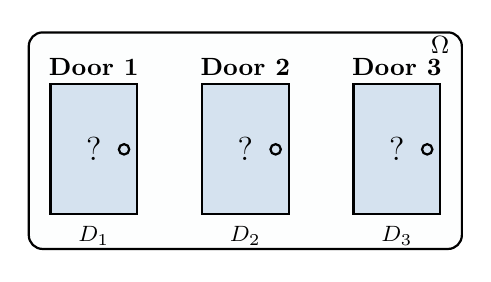
\begin{tikzpicture}[scale=0.55]
  % Sample space box
  \draw[thick, fill=lightgray, fill opacity=0.2, rounded corners=5pt] (-0.5, -0.8) rectangle (9.5, 4.2);
  \node at (9, 3.9) {\small $\Omega$};

  % Door 1
  \draw[thick, fill=ocean!20] (0, 0) rectangle (2, 3);
  \draw[thick] (1.7, 1.5) circle (0.12);
  \node at (1, 3.4) {\small\textbf{Door 1}};
  \node at (1, 1.5) {\large ?};
  \node at (1, -0.5) {\footnotesize $D_1$};

  % Door 2
  \draw[thick, fill=ocean!20] (3.5, 0) rectangle (5.5, 3);
  \draw[thick] (5.2, 1.5) circle (0.12);
  \node at (4.5, 3.4) {\small\textbf{Door 2}};
  \node at (4.5, 1.5) {\large ?};
  \node at (4.5, -0.5) {\footnotesize $D_2$};

  % Door 3
  \draw[thick, fill=ocean!20] (7, 0) rectangle (9, 3);
  \draw[thick] (8.7, 1.5) circle (0.12);
  \node at (8, 3.4) {\small\textbf{Door 3}};
  \node at (8, 1.5) {\large ?};
  \node at (8, -0.5) {\footnotesize $D_3$};
\end{tikzpicture}
\end{center}

\vspace{0.2em}

The events $D_1$, $D_2$, $D_3$ (``money behind door $i$'') are \highlight{mutually exclusive} and \highlight{exhaustive}. With no information, each is equally likely:

\vspace{-0.3em}
\[
\Prob(D_1) = \Prob(D_2) = \Prob(D_3) = \frac{1}{3} \qquad \text{\deemph{(the \textbf{prior})}}
\]

\end{frame}

% ----------------------------------------------------------------------------

\begin{frame}
\frametitle{The Monty Hall Problem}
\framesubtitle{Step 2: You choose}

\textbf{You pick Door 1.} Since the doors are equally likely, it doesn't matter which you choose.

\vspace{0.2em}

\begin{center}
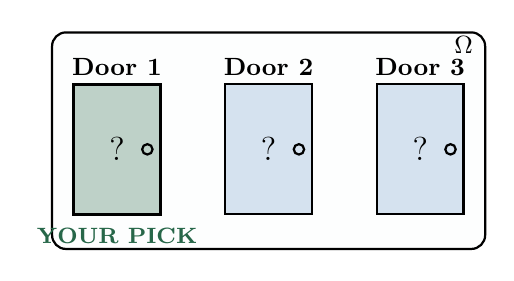
\begin{tikzpicture}[scale=0.55]
  % Sample space box
  \draw[thick, fill=lightgray, fill opacity=0.2, rounded corners=5pt] (-0.5, -0.8) rectangle (9.5, 4.2);
  \node at (9, 3.9) {\small $\Omega$};

  % Door 1 - selected (highlighted)
  \draw[very thick, fill=forest!30] (0, 0) rectangle (2, 3);
  \draw[thick] (1.7, 1.5) circle (0.12);
  \node at (1, 3.4) {\small\textbf{Door 1}};
  \node at (1, 1.5) {\large ?};
  \node at (1, -0.5) {\footnotesize\textcolor{forest}{\textbf{YOUR PICK}}};

  % Door 2
  \draw[thick, fill=ocean!20] (3.5, 0) rectangle (5.5, 3);
  \draw[thick] (5.2, 1.5) circle (0.12);
  \node at (4.5, 3.4) {\small\textbf{Door 2}};
  \node at (4.5, 1.5) {\large ?};

  % Door 3
  \draw[thick, fill=ocean!20] (7, 0) rectangle (9, 3);
  \draw[thick] (8.7, 1.5) circle (0.12);
  \node at (8, 3.4) {\small\textbf{Door 3}};
  \node at (8, 1.5) {\large ?};
\end{tikzpicture}
\end{center}

\vspace{0.1em}

At this point, what's the probability you picked the winning door?

\vspace{-0.5em}
\[
\Prob(D_1) = \frac{1}{3} \qquad \Prob(D_2 \cup D_3) = \frac{2}{3}
\]

\vspace{-0.7em}
\deemph{You have a 1/3 chance of being right. The money is \emph{more likely} behind one of the other two doors.}

\end{frame}

% ----------------------------------------------------------------------------

\begin{frame}
\frametitle{The Monty Hall Problem}
\framesubtitle{Step 3: Monty opens a door}

\textbf{Monty Hall}, the host, \emph{knows} where the money is. He opens Door 2: a goat.

\vspace{0.2em}

\begin{center}
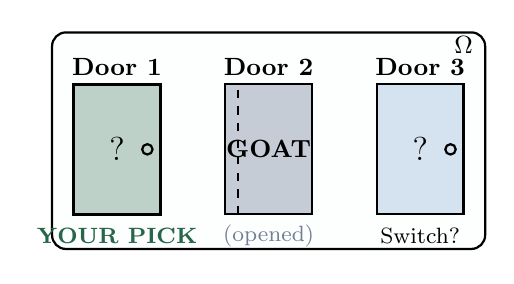
\begin{tikzpicture}[scale=0.55]
  % Sample space box
  \draw[thick, fill=lightgray, fill opacity=0.2, rounded corners=5pt] (-0.5, -0.8) rectangle (9.5, 4.2);
  \node at (9, 3.9) {\small $\Omega$};

  % Door 1 - your pick
  \draw[very thick, fill=forest!30] (0, 0) rectangle (2, 3);
  \draw[thick] (1.7, 1.5) circle (0.12);
  \node at (1, 3.4) {\small\textbf{Door 1}};
  \node at (1, 1.5) {\large ?};
  \node at (1, -0.5) {\footnotesize\textcolor{forest}{\textbf{YOUR PICK}}};

  % Door 2 - opened, showing goat
  \draw[thick, fill=warmgray!40] (3.5, 0) rectangle (5.5, 3);
  \draw[thick, dashed] (3.8, 0) -- (3.8, 3);
  \node at (4.5, 3.4) {\small\textbf{Door 2}};
  \node at (4.5, 1.5) {\small\textbf{GOAT}};
  \node at (4.5, -0.5) {\footnotesize\textcolor{warmgray}{(opened)}};

  % Door 3
  \draw[thick, fill=ocean!20] (7, 0) rectangle (9, 3);
  \draw[thick] (8.7, 1.5) circle (0.12);
  \node at (8, 3.4) {\small\textbf{Door 3}};
  \node at (8, 1.5) {\large ?};
  \node at (8, -0.5) {\footnotesize Switch?};
\end{tikzpicture}
\end{center}

\vspace{0.2em}

Monty asks: \emph{``Would you like to switch to Door 3?''}

\vspace{0.3em}

\highlight{The question}: Has the probability changed? Is $\Prob(D_3 \mid O) = \frac{1}{3}$ still, or has Monty's action given us new information?

\end{frame}

% ----------------------------------------------------------------------------

\begin{frame}
\frametitle{The Monty Hall Problem}
\framesubtitle{The key insight}

\vspace{0.3em}

\highlight{Key}: Monty's choice is \emph{not random}---it's constrained by his knowledge.

\vspace{0.5em}

\begin{itemize}
\item Monty \emph{knows} where the money is
\item Monty will \emph{never} open the door with the money
\item Monty will \emph{never} open the door you picked
\end{itemize}

\vspace{0.5em}

This means his action \highlight{reveals information}. We need to update our beliefs.

\vspace{0.5em}

Let $O$ = ``Monty opened door 2.'' We want to compute:
\[
\Prob(D_3 \mid O) = \text{?}
\]

\deemph{Is this still $\frac{1}{3}$, or has it changed? Let's use Bayes' Rule to find out.}

\end{frame}

% ----------------------------------------------------------------------------

\begin{frame}
\frametitle{The Monty Hall Problem}
\framesubtitle{Setting up Bayes' Rule}

\vspace{0.5em}

We want $\Prob(D_3 \mid O)$ using Bayes' Rule:

\vspace{0.5em}

\[
\Prob(D_3 \mid O) = \frac{\Prob(O \mid D_3) \cdot \Prob(D_3)}{\Prob(O \mid D_1)\Prob(D_1) + \Prob(O \mid D_2)\Prob(D_2) + \Prob(O \mid D_3)\Prob(D_3)}
\]

\vspace{0.5em}

\textbf{Priors}: $\Prob(D_1) = \Prob(D_2) = \Prob(D_3) = \frac{1}{3}$

\end{frame}

% ----------------------------------------------------------------------------

\begin{frame}
\frametitle{The Monty Hall Problem}
\framesubtitle{The likelihoods}

\vspace{0.5em}

\textbf{Key insight}: Monty \emph{knows} where the money is and will \emph{never} open a door with money.

\vspace{1em}

What is $\Prob(O \mid D_i)$? (Given the money is behind door $i$, what's the probability Monty opens door 2?)

\vspace{0.5em}

\begin{enumerate}
\item $\Prob(O \mid D_1) = 0.5$
\\ \deemph{Money behind door 1. Monty can choose door 2 or 3 randomly.}

\vspace{0.3em}

\item $\Prob(O \mid D_2) = 0$
\\ \deemph{Money behind door 2. Monty would never open door 2!}

\vspace{0.3em}

\item $\Prob(O \mid D_3) = 1$
\\ \deemph{Money behind door 3. Monty must open door 2 (can't open door 1 or 3).}
\end{enumerate}

\end{frame}

% ----------------------------------------------------------------------------

\begin{frame}
\frametitle{The Monty Hall Problem}
\framesubtitle{The calculation}

\vspace{0.5em}

\[
\Prob(D_3 \mid O) = \frac{\Prob(O \mid D_3) \cdot \Prob(D_3)}{\Prob(O \mid D_1)\Prob(D_1) + \Prob(O \mid D_2)\Prob(D_2) + \Prob(O \mid D_3)\Prob(D_3)}
\]

\vspace{0.5em}

Substituting:

\[
\Prob(D_3 \mid O) = \frac{1 \cdot \frac{1}{3}}{\frac{1}{2} \cdot \frac{1}{3} + 0 \cdot \frac{1}{3} + 1 \cdot \frac{1}{3}}
\]

\[
= \frac{\frac{1}{3}}{\frac{1}{6} + 0 + \frac{1}{3}} = \frac{\frac{1}{3}}{\frac{1}{2}} = \textcolor{forest}{\frac{2}{3}}
\]

\end{frame}

% ----------------------------------------------------------------------------

\begin{frame}
\frametitle{The Monty Hall Problem}
\framesubtitle{The answer}

\vspace{1em}

\begin{center}
\Large
$\Prob(D_3 \mid O) = \frac{2}{3}$ \qquad $\Prob(D_1 \mid O) = \frac{1}{3}$
\end{center}

\vspace{1.5em}

\highlight{Definitely switch to door 3!}

\vspace{1em}

\textbf{Intuition}:
\begin{itemize}
\item When you picked door 1, you had a $\frac{1}{3}$ chance of being right
\item The other two doors collectively had $\frac{2}{3}$ probability
\item Monty's action \emph{concentrates} that $\frac{2}{3}$ onto door 3
\end{itemize}

\vspace{0.5em}

\deemph{Marilyn vos Savant was right. The angry PhDs were wrong. Bayes' Rule settles it.}

\end{frame}

% ----------------------------------------------------------------------------

\begin{frame}
\frametitle{Bayes and Strategic Behavior}
\framesubtitle{When actions reveal information}

In Monty Hall, the host's action (opening door 2) \highlight{reveals information} because it's constrained by what he knows. This is the foundation of \highlight{signaling theory}:

\vspace{0.3em}

\begin{itemize}
\item \textbf{Michael Spence (1973)}: Education as a signal of ability. If degrees are \emph{easier} for high-ability workers, employers can use education to update beliefs. \deemph{(Nobel Prize, 2001)}
\item \textbf{Amotz Zahavi (1975)}: The peacock's tail is \emph{costly}---only fit males can afford it. Costly signals are credible.
\item \textbf{Diego Gambetta (2009)}: Criminals use tattoos and rituals as costly signals of commitment. \deemph{(\emph{Codes of the Underworld})}
\end{itemize}

\vspace{0.3em}

\deemph{In game theory, we solve for \highlight{Perfect Bayesian Equilibrium}: strategies are optimal given beliefs, and beliefs are updated via Bayes' Rule. David Lewis discovered signaling in his 1969 dissertation---before Spence.}

\end{frame}

% ----------------------------------------------------------------------------

\begin{frame}
\frametitle{Bayes' Rule in Action}
\framesubtitle{Medical testing example (we'll work through this together)}

\vspace{0.8em}

\textbf{Classic application}: A medical test for a rare disease.

\vspace{0.3em}

\begin{itemize}
\setlength{\itemsep}{2pt}
\item Tests have \highlight{sensitivity} (true positive rate) and \highlight{specificity} (true negative rate)
\item But what we really want is: given a positive test, what's $\Prob(\text{disease} \mid \text{positive})$?
\item This requires \emph{flipping} the conditional---exactly what Bayes' Rule does
\end{itemize}

\vspace{0.5em}

\textbf{Key ingredients}:
\begin{itemize}
\setlength{\itemsep}{2pt}
\item The \highlight{prior}: How common is the disease? (base rate)
\item The \highlight{likelihoods}: How good is the test at detecting disease/non-disease?
\end{itemize}

\vspace{0.8em}

\highlight{Let's work through a specific example on the board...}

\vspace{0.3em}

\deemph{Base rates matter. When people ignore priors, this is called the ``base rate fallacy.''}

\end{frame}

% ----------------------------------------------------------------------------
% WHY INDEPENDENCE MATTERS
% ----------------------------------------------------------------------------

\begin{frame}
\frametitle{Why Independence Matters}

\vspace{1em}

Independence dramatically simplifies calculations:

\vspace{0.5em}

\begin{itemize}
\item $\Prob(A \cap B) = \Prob(A) \cdot \Prob(B)$ (no need to find conditional)
\vspace{0.3em}
\item For $n$ independent events: $\Prob(A_1 \cap \cdots \cap A_n) = \prod_{i=1}^{n} \Prob(A_i)$
\end{itemize}

\vspace{1em}

\textbf{In this course}:

\vspace{0.5em}

\begin{itemize}
\item The \highlight{i.i.d.\ assumption} (coming in a few weeks) assumes observations are independent
\item Many of our results depend on independence
\item When independence fails, we need different tools (clustering, time series)
\end{itemize}

\end{frame}

% ----------------------------------------------------------------------------
% RECAP AND LOOKING AHEAD
% ----------------------------------------------------------------------------

\begin{frame}
\frametitle{Today's Key Ideas}

\vspace{0.5em}

\begin{enumerate}
\item \textbf{Sample spaces and events}: The vocabulary for describing outcomes
\vspace{0.5em}
\item \textbf{Kolmogorov axioms}: Non-negativity, normalization, additivity
\vspace{0.5em}
\item \textbf{Conditional probability}: $\Prob(A \mid B) = \Prob(A \cap B) / \Prob(B)$
\vspace{0.5em}
\item \textbf{Independence}: $\Prob(A \cap B) = \Prob(A)\Prob(B)$
\vspace{0.5em}
\item \textbf{Law of Total Probability}: Follows from additivity axiom
\vspace{0.5em}
\item \textbf{Bayes' Rule}: Derived from conditional probability; flips conditionals
\end{enumerate}

\vspace{1em}

\deemph{This is the language. Next: the objects we'll actually work with.}

\end{frame}

% ----------------------------------------------------------------------------

\begin{frame}
\frametitle{Looking Ahead}

\vspace{1em}

\textbf{Wednesday}: Conditional probability and Bayes' Rule (continued)

\vspace{0.5em}

\begin{itemize}
\item More examples of Bayes' Rule
\item Law of Total Probability applications
\end{itemize}

\vspace{1em}

\textbf{Next week}: Random variables, expectation, and variance

\vspace{0.5em}

\textbf{Week 3}: Famous distributions (two full lectures)

\vspace{0.5em}

\deemph{We're building the vocabulary to describe populations precisely.}

\end{frame}

% ----------------------------------------------------------------------------

\begin{frame}
\frametitle{For Wednesday}

\vspace{1em}

\textbf{Reading}:
\begin{itemize}
\item Aronow \& Miller, \S 1.1: Review today's material
\item Blackwell, Chapter 2.1: Probability foundations
\end{itemize}

\vspace{1em}

\textbf{Think about}:
\begin{itemize}
\item In the medical testing example, what would happen if prevalence were 10\% instead of 1\%?
\item Can you think of real-world examples where base rate neglect causes problems?
\end{itemize}

\vspace{1.5em}

\begin{center}
\large
\textcolor{forest}{Questions?}
\end{center}

\end{frame}

% ============================================================================
\end{document}
% ============================================================================
